\subsection{Wprowadzenie do detekcji obiektów}
Detekcja obiektów to podstawowe zadanie dziedziny wizji komputerowej, które objejmuje klasyfikowanie oraz lokalizowanie obiektów na obrazie. W przeciwieństwie do zadania klasyfikacji obrazów, które dostarcza informacji o wykrytych klasach obiektów, detekcja obiektów zapewnia zarówno klasyfikację, jak i lokalizację przestrzenną. Detekcja obiektów znajduje zastosowanie w wielu obszarach, takich jak: pojazdy autonomiczne \cite{pojazdy_autonomiczne}, obrazowanie w medycynie \cite{obrazowanie_w_medycynie}, monitoring wizyjny \cite{monitoring_wizyjny}, monitoring dzikiej przyrody \cite{wildlife}, zarządzanie sprzedażą detaliczną i zapasami \cite{sklepy}.

\subsection{Rozwój technik detekcji obiektów}
Wczesne metody detekcji obiektów opierały się na ręcznie zaprojektowanych cechach i tradycyjnych technikach uczenia maszynowego. Przykłady obejmują rozwiązania oparte na kaskadach Haara \cite{haar} lub histogramie zorientowanych gradientów (HOG) \cite{hog}, które następnie klasyfikowano za pomocą algorytmów takich jak maszyny wektorów nośnych (SVM) \cite{svm}. Ówcześnie podejścia te były przełomowe, wymagały jednak dużych nakładów obliczeniowych.

Zastosowanie uczenia głębokiego zrewolucjonizowało detekcję obiektów, a konwolucyjne sieci neuronowe (CNN) stały się podstawą nowoczesnych metod. Punktem przełomowym było pojawienie się tzw. CNN opartej na regionach (R-CNN) w 2014 r. \cite{RCNN}. Kolejne modele z rodziny R-CNN, opublikowane do 2016 r., to \emph{Fast R-CNN} \cite{Fast-RCNN} oraz \emph{Faster R-CNN} \cite{Faster-RCNN}.
\begin{figure}[H]
    \centering
    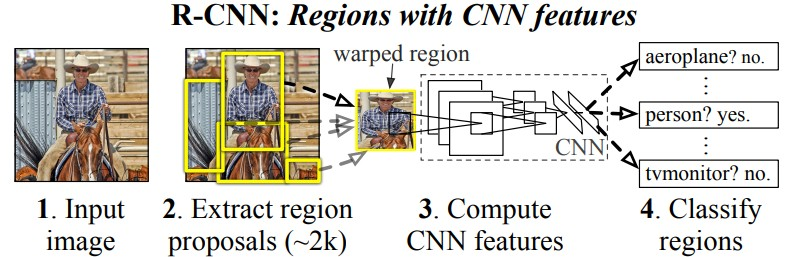
\includegraphics[width=\linewidth]{r_technologie/AI_assets/rcnn.png}
    \caption{Zarys działania modelu R-CNN. Źrodło: rozdział \emph{1. Introduction} w \cite{RCNN}}.
    \label{fig:R-CNN-schemat}
\end{figure}

Uprosczony schemat działania modelu R-CNN można przedstawić następująco:
\begin{enumerate}
    \item \textbf{Propozycja regionów:} Generowana jest pewna liczba regionów na obrazie wejściowym. Region to obszar obrazu, w którym potencjalnie może znajdować się wykrywany typ obiektu.
    \item \textbf{Pozyskanie cech regionów:} Każdy region jest odpowiednio przeskalowywany, a następnie przetwarzany za pomocą konwolucyjnej sieci neuronowej (CNN) w celu pozyskania wektora cech o stałym rozmiarze.
    \item \textbf{Klasyfikacja obiektów:} Na podstawie uzyskanego wektora cech odbywa się klasyfikacja każdego regionu -- przypisanie lub nie klasy obiektu do każdego regionu. Na koniec obszary regionów są poprawiane, aby lepiej obramowywały wykryty obiekt, a także usuwane są niektóre nachodzące na siebie regiony. Wynikowe regiony często określa się mianem prostokątów ograniczających (ang. \emph{bounding boxes}).
\end{enumerate}

 Koncepcja regionów znacznie zwiększyła dokładność detekcji (źródło: badania opisane w \cite{RCNN, Fast-RCNN, Faster-RCNN}), aczkolwiek modele z tej rodziny -- pomimo postępów w nowszych wersjach -- nadal były stosunkowo wolne ze względu na ich wieloetapowy schemat działania. Modele z rodziny R-CNN można okreslić mianem detektorów dwuetapowych (ang. \emph{two-stage detectors}), ponieważ w sposób niesymultaniczny wykonywały one dwa zadania:
\begin{enumerate}
    \item \textbf{Określenie lokalizacji:} propozycja regionów
    \item \textbf{Klasyfikacja:} pozyskanie cech regionów i klasyfikacja obiektów
\end{enumerate}

Opublikowanie w 2016 roku pierwszej wersji modelu YOLO (ang. \emph{You Only Look Once}) \cite{yolo_pierwszy_artykul} stało się istotnym wydarzeniem w dziedzinie wizji komputerowej. Podstawowym założeniem modelu jest jednoczesna realizacja zadań klasyfikacji i lokalizacji w ramch tylko pojedyńczego przejścia przez sieć konwolucyjną.  
Zaproponowane rozwiązanie było przykładem tzw. detektora jednostopniowego (ang. \emph{one-stage detector}). Jednostopniowość określa się jednoczesnym wykonywaniem klasyfikacji jak i określeniem lokalizacji.

\begin{figure}[H]
    \centering
    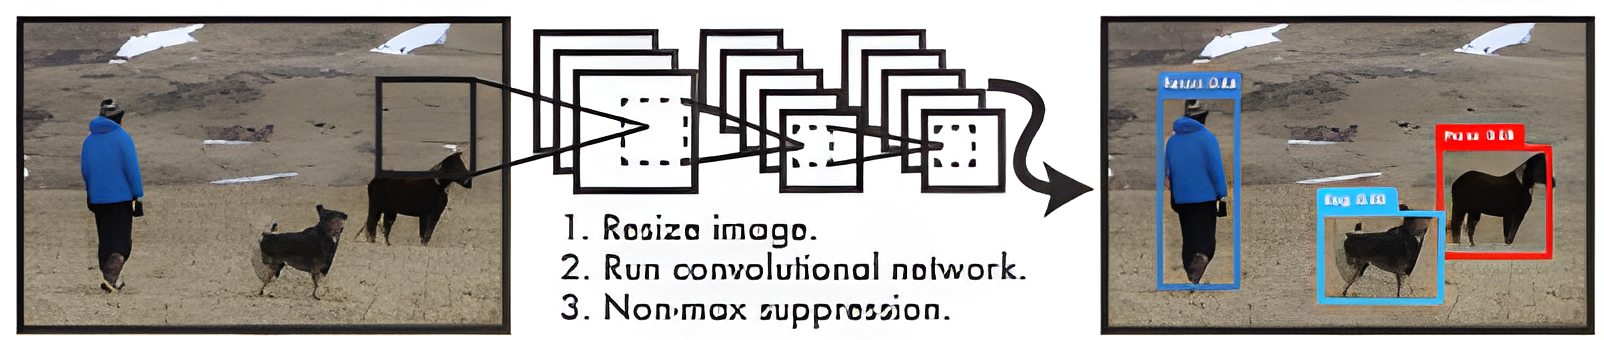
\includegraphics[width=\linewidth]{r_technologie/AI_assets/yolov1_1.png}
    \caption{Zarys działania modelu YOLOv1. Źrodło: rodział \emph{1. Introduction} w \cite{yolo_pierwszy_artykul}} .
    \label{fig:yolov1-schemat-dzialania}
\end{figure}
\begin{figure}[H]
    \centering
    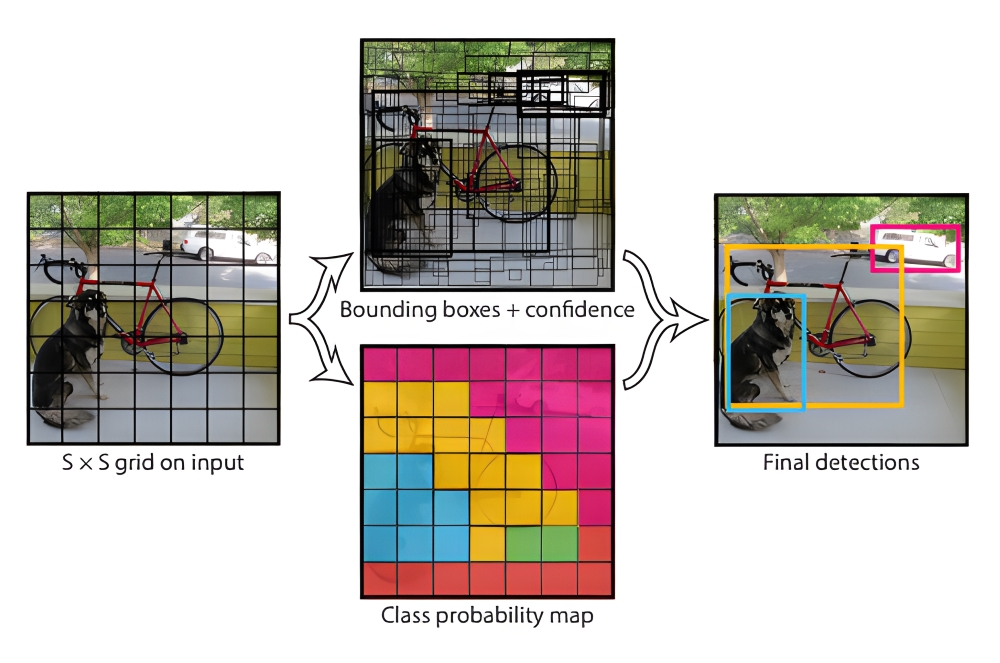
\includegraphics[width=\linewidth]{r_technologie/AI_assets/yolov1_2.jpg}
    \caption{Zarys działania CNN w modelu YOLO. Źrodło: rodział \emph{2. Unified Detection} w \cite{yolo_pierwszy_artykul}} .
    \label{fig:yolov1-schemat-dzialania-CNN}
\end{figure}


Na bazie \cite{yolo_pierwszy_artykul} ogólny schemat działania modelu YOLO (rysunek \ref{fig:yolov1-schemat-dzialania}), w tym CNN (rysunek \ref{fig:yolov1-schemat-dzialania-CNN}), można przedstawić następująco:
\begin{enumerate}
    \item \textbf{Dostosowanie obrazu wejściowego:} Obraz wejściowy jest przeskalowywany do określonego przez model rozmiaru.
    \item \textbf{Przetworzenie całego przeskalowanego obrazu przez CNN:} Na tym etapie odbywa się jednoczesna klasyfikacja oraz lokalizacja obiektów:
    \begin{enumerate}
        \item \textbf{Podział obrazu:} Obraz dzielony jest na siatkę rozmiaru $SxS$ dla pewnego $S$, tworząc $S^{2}$ komórek. 
        \item \textbf{Jednoczesna lokalizacja oraz klasyfikacja:} 
        \begin{enumerate}
            \item \textbf{Lokalizacja:} Dla każdej komórki szacowanych jest $B$ prostokątów ograniczających oraz określane są wyniki pewności (ang. \emph{confidence score}) dla każdego z nich. Wynik pewności wyraża z jakim prawdopodobieństwem model stwierdza wystąpienie obiektu oraz z jaką dokładnościa określa jego położenie przestrzenne.
            \item \textbf{Klasyfikacja:} Dla każdej komórki wyliczany jest zbiór rozmiarze $C$, gdzie $C$ odpowiada liczbie wykrywanych klas przez model. Pojedyńczy element zbioru odpowiada konkretnej klasie obiektu i zawiera wartość wyrażającą prawdopodobieństwo, iż obiekt w komórce należy do tej klasy obiektu. Prawdopodobiestwo to jest prawdopodobieństwem warunkowym -- opiera się na założeniu, że komórka przedstawia jakiś obiekt. 
        \end{enumerate}
        \item \textbf{Zakodowanie wyników obu operacji i przekazanie na wyjście CNN.}
    \end{enumerate}
    \item  \textbf{Eliminacja redundancji w wynikach CNN:} Usunięcie zbędnych prostokątów ograniczających, w tym takich nachodzących na inne. 
\end{enumerate}

Badania szybkości dotychczasowo dostępnych modeli -- w tym Faster R-CNN i YOLO -- w rozdziale \emph{4.1 Comparison to Other Real-Time Systems} \cite{yolo_pierwszy_artykul} pokazały znaczącą różnicę szybkości YOLO (YOLO i Fast YOLO) względem modeli z rodziny R-CNN na rzecz YOLO. Natomiast warto nadmienić, iż jednoczna poprawa szybkości wiązała się z redukcją dokładności modelu, co również zostało ukazane w w.w. badaniu.

Od momentu publikacji YOLO do momentu powstania niniejszego dokumentu (11 grudnia 2024) można wyróżnić co najmiej dziewięć kolejnych modeli. Modele te dokonywały różne zmiany w architekturze modelu pierwotnego, niemniej każdy z nich zachował podstawowe założenie realizacji zadań detekcji obiektów poprzez tylko pojedyńcze przejście przez CNN. 

Wizja komputerowa rozwija się w sposób dynamiczny. Na stan aktualny (grudzień 2024), w obecnym roku można wyróżnić co najmniej trzy nowe wersje modelu, w tym YOLO11 \cite{yolo11_ultralytics} (źródło: dokumentacja od firmy \emph{Ultralytics} \cite{yolo_docs}, podstrona \emph{/models}).
Ze względu na dynamikę rozwoju, w chwili wyboru wersjii dla niniejszego systemu, postanowiono rozważyć modele opublikowane do końca 2023r.. Na podstawie porównania modeli przedstawionych w \cite{yolo_docs} (podstrona \emph{/models/yolov8}) zdecydowano o wyborze technologii YOLOv8, a konkretniej modelu YOLOv8n. Zaletą YOLOv8 jest możliwość wyboru kilku podwersji o różnym rozmiarze modelu -- im mniejszy model, tym szybszy, a jednocześnie mniej dokładny.

\begin{figure}[H]
    \centering
    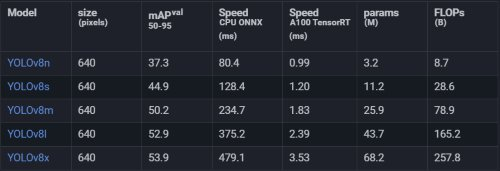
\includegraphics[width=\linewidth]{r_technologie/AI_assets/yolo8_sizes.jpg}
    \caption{Porównanie YOLOv8 o różnych rozmiarach. Wiersze posortowane wzlędem rozmiaru modelu. Źródło: \cite{yolo_docs}, podstrona \emph{/models/yolov8}}.
    \label{fig:yolo8-sizes}
\end{figure}

Ponieważ zaprojektowany system będzie operował na sprzęcie komputerowym (z naciskiem na kartę graficzną) posiadanym przez przeciętnego użytkownika, zdecydowano się postawić na szybkość modelu --- stąd wybór YOLOv8n. Zaletą YOLOv8 jest również duża liczba dostępnych klas obiektów dla niedostrojonego (ang. \emph{fine-tuned}) modelu -- jest ich 80. Zbiór dostępnych klas bazuje na zestawie danych COCO \cite{COCO_docs}. 

Podsumowując, użytym modelem w tym projekcie będzie podstawowa, niedostrojona wersja YOLOv8n. 



\subsection{Interfejs programistyczny do YOLO od firmy Ultralytics}
\label{chap:wprowadzenie-yolo_interjes}
Firma Ultralytics dostarcza interfejs programistyczny w formie pobieralnego modułu do języka Python \cite{Python_docs}. Poprzez różne tryby interfejsu istnieje możliwość wykorzystania różnego aspektu modelu. 

Tryby użytkowania to między innymi (źródło \cite{yolo_docs}, podstrona \emph{/modes}):
\begin{itemize}
    \item \textbf{train}: tryb do trenowania modelu na innych zestawach danych.
    \item \textbf{predict}: tryb inferencji. W kontekście YOLO, inferencja oznacza detekcję obiektów.
    \item \textbf{val}: tryb używany do ewaluacji przetrenowanego modelu.
\end{itemize}

W projeckie użyto trybu inferencji. Warto wspomnieć, iż dokumentacja \cite{yolo_docs} jest, na chwilę obecną (2 grudnia 2024), często pisana z perspektywy modelu YOLOv11. W praktyce wiele funkcji interfejsu działa również na innych wersjach modelu, w tym wersjach opartych na otwartym oprogamowaniu, a nie będących jednocześnie stworzonych przez autorów interfejsu. W przypadku użytych funkcji trybu inferencji, nie pojawiły się żadne problemy przy próbie użycia dla modelu YOLOv8n. 


\begin{lstlisting}[caption={Użycie trybu inferencji na przykładzie własnego kodu źródłowego.}, label={lst:inference_interface}]
from cv2.typing import MatLike
from ultralytics import YOLO
from ultralytics.engine.results import Results

from detector.yolo_settings import yolo_inference_config


class ImageProcessor:
    def __init__(self) -> None:
        self._detector = YOLO('yolo_models/yolov8.pt')

    def detect_objects(self, frame: MatLike) -> Tuple[Results, bool]:
        results = self._detector.predict(
            frame,
            conf=yolo_inference_config.confidence_threshold,
            device=yolo_inference_config.device,
            classes=yolo_inference_config.classes,
            verbose=yolo_inference_config.verbose
        ) # Returned type: list[Results] with only one element
        first_frame_result = results[0] # Get first (and only) frame from the list

        # Return detection results and also if there were any detected objects
        return first_frame_result, len(first_frame_result.boxes) > 0 

     def visualize_objects_presence(self, frame: MatLike, detections: Results) -> Tuple[MatLike, bool]:
        for box in detections.boxes:
            # Visualize bounding boxes
            x_min, y_min, x_max, y_max = box.xyxy[0] # coordinates
            # ...
\end{lstlisting}

Na bazie kodu \ref{lst:inference_interface}, inferencji można dokonać w następujący sposób:
\begin{itemize}
    \item \textbf{Zaimportowanie odpowiedniego obiektu z modułu ultralytics:} Aby skorzystać z usług interfejsu do komunikacji z modelami YOLO, wystarczy zaimportować i użyć obiekt \emph{YOLO} --- \emph{from ultralytics import YOLO}. Następnie należy stworzyć instancje wybranej przez użytkownika i dostępnej wersji YOLO, w tym wypadku YOLOv8 --- \emph{YOLO('yolo\_models/yolov8.pt')}.

    \item \textbf{Uzycie inferencji:} Inferencję można wykonać wywołaniem tylko jednej metody na wcześniej stworzonej instancji modelu --- metoda \emph{predict}. Pierwszy argument jest obowiązkowy, i jest źródłem obrazu. W tym przypadku jako argument podano klatkę obrazu pobraną przez bilbiotekę OpenCV -- typ \emph{MatLike}. Dalsze argumenty są opcjonalne. W przypadku niniejszego projektu użyto czterech z nich:
    \begin{itemize}
        \item \textbf{conf:} Parametr filtrujący. Jest to tzw. próg ufności (ang. \emph{confidence threshold}) wyrażony liczbą całkowitą z przedziału $[0.00, 1.00]$. Każda detekcja o wyniku pewności detekcji o wartości mniejszej od tego parametru jest odrzucana. 
        \item \textbf{device:} Określa urządzenie, na którym przeprowadzana jest inferencja. W projekcie tym użyto opcji \emph{'cuda'} --- inferencja przeprowadzana jest na procesorze graficznym firmy Nvidia.
        \item \textbf{classes:} Parametr filtrujący. Jest wyrażany listą indeksów klas obiektów. Określa klasy obiektów, których wykrycia model ma zwracać.
        Użycie tego parametru filtruje wyniki inferencji i zwraca wystąpienia tylko podanych klas. 
        \item \textbf{verbose:} Przyjmuje \emph{true} albo \emph{false}. Określa czy informacje na temat inferencji będą wysyłane do ustawionego strumienia wyjściowego. Parametr będzie zawsze ustawiony na \emph{false}.
    \end{itemize}
    Wyniki inferencji są zwracane jako typ \emph{Results}. Zawiera on m.in. liste prostokątów ograniczających. Pobranie koordynatów prostokąta dla pojedyńczego wyniku wymaga jedynie iteracji przez liste prostokątów (\emph{detections.boxes}) a następnie pobrania koordynatów z pojedyńczego prostokąta (\emph{box.xyxy[0]}).
\end{itemize}

W celu znalezienia informacji o pracy z obiektem wynikowym \emph{Results} oraz zapoznania się z resztą dostępnych parametrów inferencji rekomenduje się podstronę \emph{modes/predict} dokumentacji \cite{yolo_docs}.

Przedstawiony interfejs w przejrzysty i prosty sposób pozwala na użytkowanie modelu YOLOv8n. Jest to kolejny powód wybrania właśnie tej technologii. 

Niniejszy system umożliwia zmianę wartości progu ufności (\emph{conf}) oraz wykrywanych klas (\emph{classes}).

Warto również wspomnieć o parametrze \emph{imgsz}. Określa on rozmiar obrazu, na którym jest przeprowadzona detekcja obiektów. Obraz wejściowy jest przeskalowywany do tego rozmiaru. W projekcie wykorzystano domyślną wartość parametru, równą 640x640px.